\begin{frame}
	\manimate
	\frametitle{Алгоритми}
	\begin{enumerate}
		\item Віднімання фону ( медіана, Гауса )
		\item Байесовський класифікатор \\
		\begin{enumerate} 
			\item Класична реалізація
			\item Поправки ймовірностей
			\item Удосконалений метод навчання
		\end{enumerate}
		\item Розпізнавання на основі сенсора глибини ( Intel Realsense F200 camera)
	\end{enumerate}
	
\end{frame}

\begin{frame}
	\manimate
	\frametitle{Віднімання фону}
	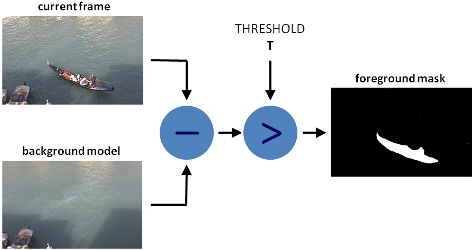
\includegraphics[width=1.0\linewidth]{im/background_substraction}
\end{frame}

\begin{frame}
	\manimate
	\frametitle{Байесовський класифікатор}
	\begin{equation}
		P(s|c) = \frac{P(c|s) * P(s)}{P(c)}
	\end{equation}
\end{frame}

\begin{frame}
	\manimate
	\frametitle{Відеопотік камери глибини}
	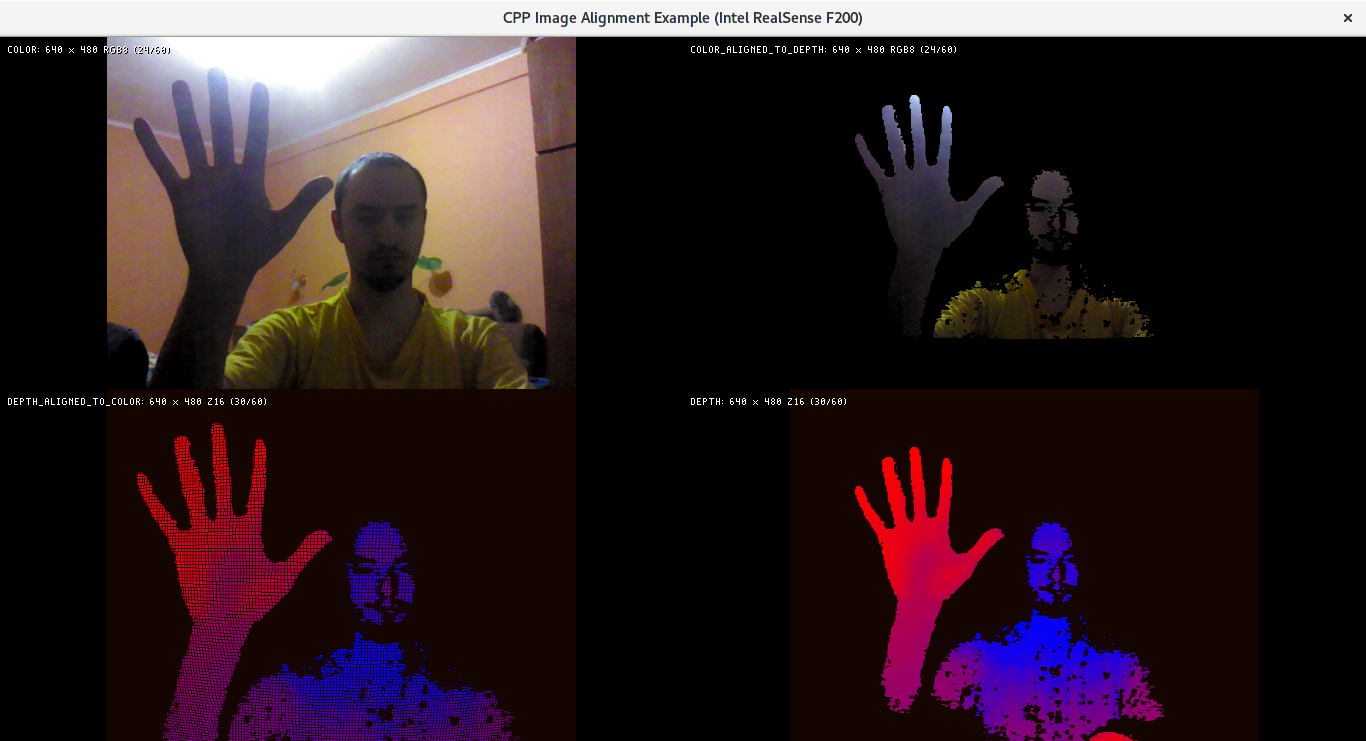
\includegraphics[width=1.0\linewidth]{im/depth_camera}
\end{frame}